\documentclass[oneside,12pt]{book}
% oneside - onesided print

%\usepackage[czech]{babel}
\usepackage[utf8]{inputenc}
\usepackage[a4paper,width=150mm,top=25mm,bottom=30mm]{geometry}
\usepackage[backend=biber,style=numeric,sorting=none]{biblatex}
\usepackage{setspace, enumitem, amsmath, amsfonts, amsthm, amssymb, graphicx, soul, float, multirow, hyperref}
\usepackage{xcolor, listings, csquotes, wrapfig}

% Page number at the end of page and no chapter name in the header
\pagestyle{plain}

\setstretch{1.5}

\setcounter{secnumdepth}{3}

\bibliography{references}

\definecolor{keywords}{rgb}{0,0,0.7}

\lstset{
columns=fullflexible,
keywordstyle=\color{keywords},
frame=lines,
language=Python,
%numbers=left,
%numbersep=5pt,
basicstyle=\small,
%numberstyle=\footnotesize\color{Gray},
commentstyle=\it\footnotesize\color{Gray}
}

\newenvironment{boldenv}{\bfseries}{}

\newcommand\norm[1]{\left\lVert#1\right\rVert}

\theoremstyle{definition}
\newtheorem{defn}{Definition}[section]

\DeclareMathOperator*{\argmax}{arg\,max}
\DeclareMathOperator*{\argmin}{arg\,min}

\begin{document}
    \pagenumbering{gobble}

    \begin{titlepage}
    \begin{boldenv}
        \begin{center}
            \vspace*{20pt}
            \LARGE
            University of West Bohemia \\
            \vspace*{5pt} Faculty of Applied Sciences  \\
            \vspace*{5pt} Department of Cybernetics\\

            \vfill
            \huge
            MASTER THESIS

            \vfill

        \end{center}
        \begin{flushleft}
            \Large
            PILSEN, 2020
            \hfill
            JAN BENEŠ
        \end{flushleft}
    \end{boldenv}
\end{titlepage}

    Před svázáním místo této stránky \fbox{vložit zadání práce} s podpisem děkana.
    \newpage

    \vspace*{20pt}
\begin{center}
    \underline{Declaration of Authorship}
\end{center}

I, Jan Beneš, declare that this thesis titled, “Automatic face recognition using neural networks” and the work 
presented in it are my own.

I confirm that:
\begin{itemize}
    \item Where I have consulted the published work of others, this is always clearly attributed.
    \item Where I have quoted from the work of others, the source is always given.
    With the exception of such quotations, this thesis is entirely my own work.
    \item I have acknowledged all main sources of help.
\end{itemize}

    \newpage

    \vspace*{20pt}
\noindent
{\LARGE
\textbf{Acknowledgements}
}
\vspace*{0.5em}

I would like to express my gratitude and appreciation to Ing. Ivan Gruber for his guidance throughout the project.

Likewise, I would like to thank my supervisor Ing. Marek Hrúz, Ph.D. for providing me with invaluable feedback.

My gratitude also goes to MetaCentrum VO for allowing  me to use their computational resources.

Finally, I have to thank my family for supporting me in the pursuit of my studies.

    \section*{Abstract}
The goal of this study is to design and implement an end-to-end facial recognition system.
The first part is focused on a general overview of modern methods followed by an in-depth description of
state-of-the-art research of loss functions.
The emphasis is being put on the ArcFace loss as it is the research which forms the basis of the facial recognition
system implemented in this thesis.
The second part deals with the design and implementation of the system.
The end of the text contains a comparison with a commercial algorithm.
The performance was evaluated on a dataset which was created from the recordings of evening news on the czech public
television broadcast (Česká Televize).

\vspace{1cm}

\subsection*{Key words}
Machine learning, facial recognition, identification, verification, convolutional neural networks, loss functions,
ArcFace

\vfill

\section*{Abstrakt}
Cílem této práce je návrh a implementace systému rozpoznávání obličeje.
V první části je poskytnut přehled moderních metod, na který navazuje podrobný rozbor výzkumu ztrátových funkcí.
Důraz je kladen na ztrátovou funkci ArcFace.
Tato funkce byla použita při trénování modelu, jenž tvoří jádro systému implementovaného v rámci této práce.
Druhá část práce obsahuje návrh a popis implementace systému.
V závěru je systém porovnán s komerčním algoritmem.
Vyhodnocení proběhlo na datasetu, jenž byl vytvořen ze záznamu večerních zpráv České Televize.

\vspace{1cm}

\subsection*{Klíčová slova}
Strojové učení, rozpoznávání obličeje, identifikace, verifikace, konvoluční neuronové sítě, ztrátové funkce, ArcFace

    \tableofcontents

    \pagenumbering{arabic}

    \chapter{Introduction}\label{ch:introduction}

\section{Objectives}\label{sec:objectives}
The objectives of this text are:
\begin{enumerate}
    \item to provide an overview of modern facial recognition methods;
    \item to implement the state-of-the-art algorithm;
    \item to evaluate the system's performance on appropriate benchmark dataset;
    \item to compare the results with commercial algorithm.
\end{enumerate}

\section{Outline}\label{sec:outline}

    \chapter{Convolutional Neural Networks}\label{ch:cnn}
Convolutional Neural Networks (CNNs) are a group of models which allow for efficient training on high dimensional data.
This is especially useful in the field of computer vision as image data is fundamentally high dimensional.

\begin{figure}[H]
    \centering
    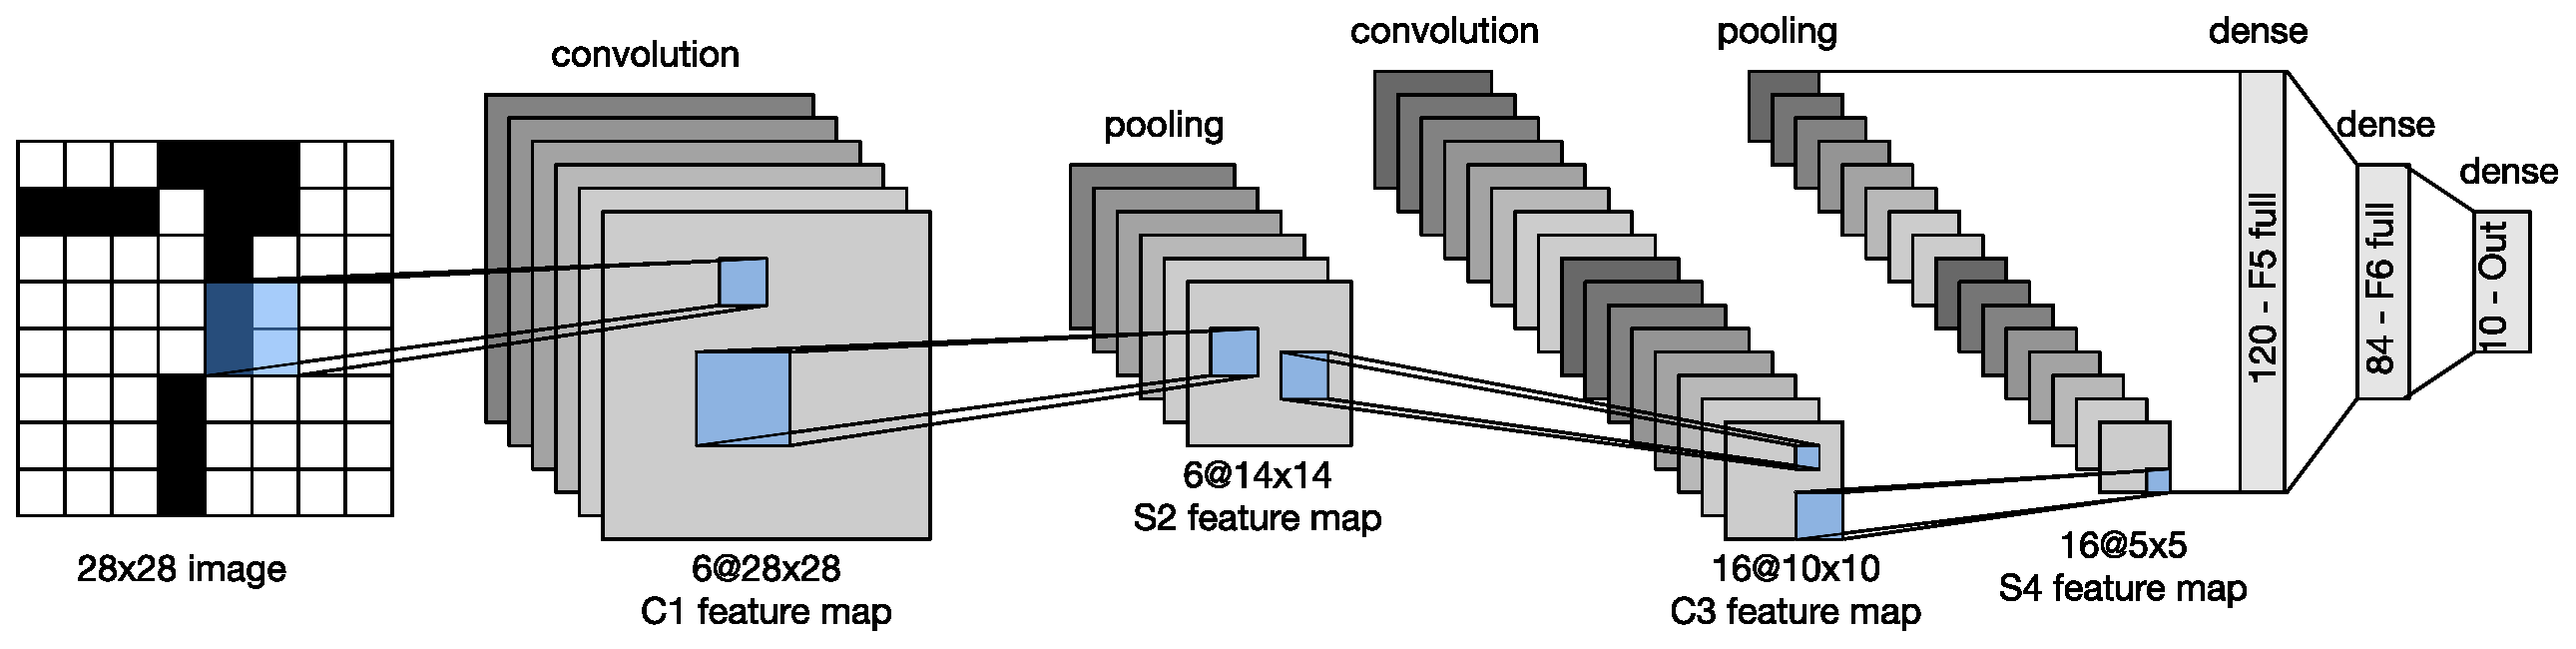
\includegraphics[width=\columnwidth]{images/cnn/lenet.eps}
    \caption{Example of CNN model (LeNet 5)~\cite{CNN}}
    \label{fig:cnn}
\end{figure}

The image~\ref{fig:cnn} is an illustration of one of the oldest CNN models \textit{LenNet 5} which was used for
handwritten character recognition.
As we can see, there are many layers stacked in the model's architecture.
This is typical for CNNs and it's a reason why CNNs belong to the class of machine learning methods called
\textit{deep learning}\footnote{Set of machine learning models with
\textit{credit assignment path (CAP)} higher than 2.
The CAP is the chain of transformations from input to output.}
Usually there are three layer types in the CNN model: \textit{dense}~\ref{sec:dense},
\textit{convolutional}~\ref{sec:convolutional} and \textit{pooling}~\ref{sec:pooling}.

\section{Dense layer}\label{sec:dense}
Dense layer is the simplest type of layer present in CNN models.
Its output is determined simply by multiplication of \textit{inputs} (x) with \textit{weight matrix}
(denoted V in~\ref{eq:dense}, also called kernel) and addition of \textit{bias} (u).

\begin{equation}
    \label{eq:dense}
    h[i, j] = u[i,j] + \sum_{a,b} V[i,j,a,b] \cdot x[i+a,j+b]
\end{equation}

Now let's imagine, that we have greyscale image which is 256 pixel wide and high as an input.
If we flatten the image to a vector, we get input with $256\cdot256 = 65536$ dimensions.
Even if we do aggressive reduction to 1000 hidden dimensions, we end up with ~65 million parameters.
This makes dense layer impractical when dealing with imagery and that's when convolution~\ref{sec:convolutional} comes
into play.

\section{Convolutional layer}\label{sec:convolutional}
As I hinted in the previous section, the main objective of convolutional layer is to decrease the amount of parameters
needed.
This feat was achieved by application of two principles: \textit{invariance}~\ref{subsec:invariance} and
\textit{locality}~\ref{subsec:locality}.

\subsection{Invariance principle}\label{subsec:invariance}
The core of invariance principle is reuse of the weights.
This is achieved by application of the weights on one part of the image, shifting the weights by a predetermined set
of pixels (called stride) and then applying the weights again.
We can have a look at equation~\ref{eq:denseinv} too see how the original equation~\ref{eq:dense} changes.

\begin{equation}
    \label{eq:denseinv}
    h[i, j] = u + \sum_{a,b} V[a,b] \cdot x[i+a,j+b]
\end{equation}

As is to be expected, bias \textit{u} and the weight matrix \textit{V} are no longer dependent upon the image
coordinates \textit{(i, j)}.
As an example we can think of an airplane detection algorithm whose objective is to find whether there is an airplane
in arbitrary location of the scene.
We would do that by sliding one set of weights describing the airplane over the image.
The algorithm would classify the scene with high impulse response as containing the airplane.
This intuitively makes a lot of sense.

This type of invariance is called \textit{translational invariance}.

\subsection{Locality principle}\label{subsec:locality}
Another principle used in CNNs is so called \textit{locality principle}.
This principle suggests, that we do not need to look far away from \textit{(i,j)} to gain valuable information about
what is going on in that particular location.
This is achieved, mathematically speaking, by limiting \textit{a} and \textit{b} to a range $\Delta$.

\begin{equation}
    \label{eq:denseinvloc}
    h[i, j] = u + \sum_{a=-\Delta}^{\Delta} \sum_{b=-\Delta}^{\Delta} V[a,b] \cdot x[i+a,j+b]
\end{equation}

Equation~\ref{eq:denseinvloc} is the final form describing the convolution layer.

\subsection{Padding}\label{subsec:padding}
To avoid loss of information at the edges of the image we usually use a method called \textit{padding}.
This technique increases the image dimension by pixel addition around the original image.
There are few padding variants which are differentiated by the value of the new pixels.
The most common ones are \textit{zero padding} and \textit{reflective padding}.
The first mentioned type, as the name implies, sets the new pixels to zero.
The second one is more sophisticated and consists in mirroring of the neighboring pixels.

\section{Pooling layer}\label{sec:pooling}



    \chapter{Face Recognition}\label{ch:face-rec}

    \chapter{ArcFace}\label{ch:arcface}
ArcFace~\cite{ArcFace} is a research which became public in 2018 and achieved state-of-the-art results on LFW dataset.

ArcLoss is based on the equation of \textit{softmax loss}~\ref{eq:softmax}.
There are few steps separating the original and the improved version:
\begin{enumerate}
    \item First step is to fix the bias $b_j = 0$.
    \item Then we transform the logit using the dot product definition $W_j^T x_i = \norm{W_j} \norm{x_j} \cos \theta_j$
    $\theta$ is the angle between the weight $W_j$ and the feature $x_i$.
    \item In a third step we fix the individual weights $\norm{W_j} = 1$ by $l_2$ normalization
    \item We do the same for feature $x_i$ and re-scale it to $s$ where coefficient $s$ is predetermined feature scale.
    These normalization steps make the prediction depend only on the angle $\theta$.
    The embeddings are distributed on the hypersphere with a radius $s$.
\end{enumerate}

\begin{figure}[H]
    \centering
    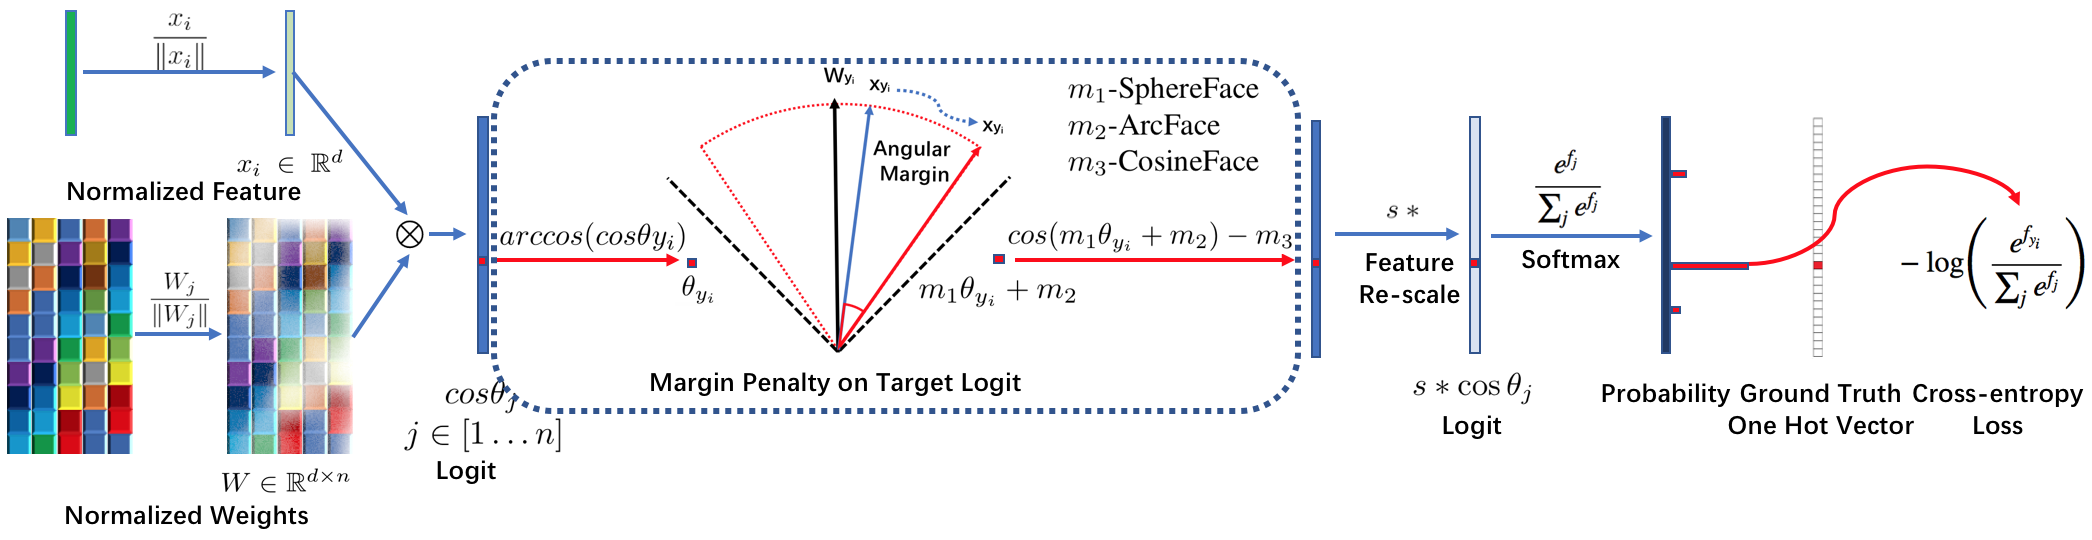
\includegraphics[width=\columnwidth]{images/arcface/arcface.png}
    \caption{Training a CNN for face recognition supervised by the ArcFace loss~\cite{ArcFace}}
    \label{fig:arcface}
\end{figure}

At this point the loss function equation is as follows:
\begin{equation}
    \mathcal{L} = -\frac{1}{N} \sum_{i=1}^{N} \log \frac{e^{s \cos(\theta_{y_i,i})}}
    {e^{s\ \cos(\theta_{y_i,i})} + \sum_{j = 1, j \neq y_i}^n e^{s\ \cos(\theta_{j,i})}}.
\end{equation}

\begin{enumerate}
    \setcounter{enumi}{4}
    \item Now we incorporate the additive margin penalty \textit{m} between $x_i$ and $W_{y_i}$.
    The angluar margin is equal to the geodesic distance\footnote{Distance of a curve representing shortest path
    between two points in a surface.} on the hypersphere which is the reason why the method is called
    \textit{ArcFace}.
\end{enumerate}

Final ArcFace loss function:
\begin{equation}
    \mathcal{L} = -\frac{1}{N} \sum_{i=1}^{N} \log \frac{e^{s \cos(\theta_{y_i,i} + m)}}
    {e^{s\ \cos(\theta_{y_i,i} + m)} + \sum_{j = 1, j \neq y_i}^n e^{s\ \cos(\theta_{j,i})}}.
\end{equation}

\section{Comparison with SphereFace and CosFace}\label{sec:arc-comparison}
By having a look at figure~\ref{fig:arcfacecomp} we can do a comparison of geometric differences of decision margins.
The advantage of \textit{ArcFace} is its constant linear angular margin throughout the whole interval.

\begin{figure}[H]
    \centering
    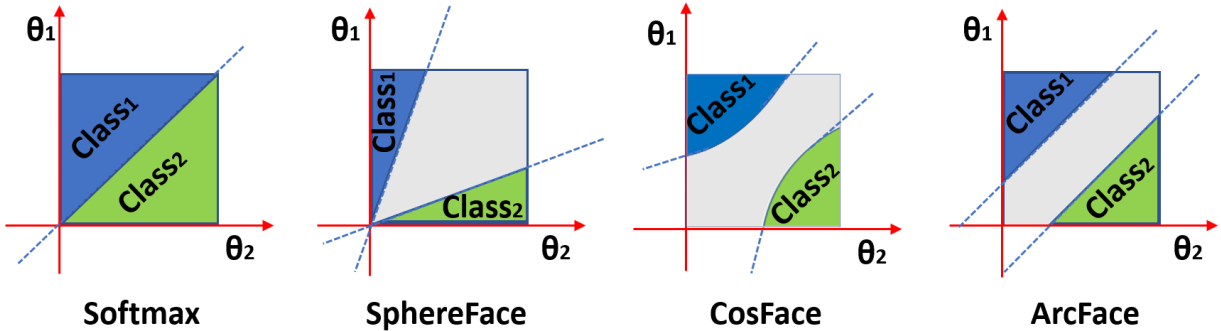
\includegraphics[width=\columnwidth]{images/arcface/arcfacecomparison.png}
    \caption{Decision margins of different loss functions under binary classification case.~\cite{ArcFace}}
    \label{fig:arcfacecomp}
\end{figure}

We can see the concrete results in table~\ref{tbl:arcfacecomp}.
ResNet100 with ArcFace loss trained on MS1MV2~\ref{subsec:ms1m} dataset exceeded the results of methods mentioned in
this thesis.

\begin{table}[H]
    \begin{tabularx}{\textwidth}{l|XXc}
        Method                & \#Image & LFW~\ref{subsec:lfw}            & YTF~\ref{subsec:ytf}            \\ \hline
        FaceNet~\ref{subsubsec:facenet}               & 200M    & 99.63          & 95.10          \\
        Center Loss~\ref{subsubsec:center-loss}           & 0.7M    & 99.28          & 94.90          \\
        SphereFace~\ref{subsubsec:sphereface-loss}            & 0.5M    & 99.42          & 95.00          \\
        CosFace~\ref{subsubsec:cosface}               & 5M      & 99.73          & 97.60          \\
        MS1MV2, R100, ArcFace & 5.8M    & \textbf{99.83} & \textbf{98.02}
    \end{tabularx}
    \caption{Verification performance (\%) of different methods on LFW and YTF datasets.}
    \label{tbl:arcfacecomp}
\end{table}

%    \setquotestyle{english} % Question marks in place of quotes bug fix
    \printbibliography

\end{document}